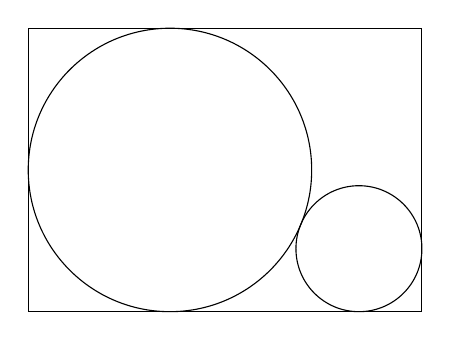
\begin{tikzpicture}
    \pgfmathsetmacro{\factor}{0.2}
    \pgfmathsetmacro{\a}{25 * \factor}% 长
    \pgfmathsetmacro{\b}{18 * \factor}% 宽

    \pgfmathsetmacro{\R}{\b/2}

    % 以长方形左下角的点为坐标原点,设大、小圆半径分别为 R、r。则:
    % 大圆圆心 A 点坐标  (R, R)
    % 小圆圆心 B 点坐标  (a - r, r)
    % 两圆相切,所以 AB 的距离 = R + r。
    % 代入两点的距离公式得
    %       sqrt{[R - (a - r)]^2 + (R - r)^2} = R + r
    % 化简后得
    %       r = (R + a) - \sqrt(4aR)
    \pgfmathsetmacro{\r}{\R + \a - sqrt(4 * \a * \R)}

    \coordinate (A) at (\R, \R);
    \coordinate (B) at (\a - \r, \r);

    \draw (0, 0) rectangle (\a, \b);
    \draw (A) circle (\R);
    \draw (B) circle (\r);
\end{tikzpicture}

